\documentclass[english,12pt]{article}

\usepackage[english]{babel}
\usepackage[utf8]{inputenc}
\usepackage[T1]{fontenc}
\usepackage{hyperref}
\usepackage{siunitx}
\usepackage{graphicx}
\usepackage{tabularx}
\usepackage{longtable}
\usepackage[hmargin=1in,vmargin=1in]{geometry}
\usepackage[dvipsnames]{xcolor}
\usepackage[normalem]{ulem}
\usepackage{flafter} 
\useunder{\uline}{\ul}{}
\begin{document}

\begin{center}

\thispagestyle{empty}

$ $

\vspace{250pt}

\begin{bfseries}

{\Large Object Recognition and Path Smoothing Robot, Phase 6}

{\Huge Test Plan}

%{\Large $\langle$application and version to be tested$\rangle$}%

\end{bfseries}

\vspace{180pt}

University of Washington Tacoma, School of Engineering and Technology

%TIE-21204 Ohjelmistojen testaus%

\vspace{12pt}

Authors: 

Ammon Dodson \href{mailto:ammon0@uw.edu}{ammon0@uw.edu} 

Alex Marlow \href{mailto:alexmarlow117@gmail.com}{alexmarlow117@gmail.com} 

Jake McKenzie \href{mailto:jake314@uw.edu}{jake314@uw.edu}

Distribution: Matthew Tolentino

Document state: draft

Modified: \today

\end{center}

\newpage


\tableofcontents

\newpage


\section{Revision History}

\begin{itemize}
	\item v0.1: In this version of the testplan we defined the  
    scope of the problem with the introduction, test items and 
    approach.
    \item v0.2: In this version of the testplan we defined the  
    test items, schedule and approach.
    \item v0.3: In this version of the testplan we updated 
    the hardware, software, and system test items with 
    tables and test descriptions. A criticality criterion 
    was added to distinguish a hierarchy of tests. Four key 
    modes were added in the hardware test items section. 
    Software test item levels were established. A figure 
    was created to show the research test environment. 
    Research testing criteria was established. The entire 
    special tools section was created with training required.
    An experts and non-experts section was established.
    Software testing methodology was established.
    \item v0.4: A section on measuring safety was established.
    A defect detection percentage was established.
    Roles were given out.
    \item v0.5: The entire schedule section was overhauled split into 
    delay handling and dates trimming much of the fluff to make it more 
    readable for the user. A regression testing section was added with three 
    criteria explored and established for introduction of regression tests.
    \item v0.6: The testing deliverables and failure criteria section was fleshed out.
    Defect detection percentage was moved to this section and a caveat was added to the 
    defined procedure as it is becoming clear that this may not be used by the end of it.
\end{itemize}


\section{Introduction}
\subsection{Purpose}
This test plan describes the testing approach and overall 
framework that will drive the testing of the ORPS-Robot 
version 0.3 – The Object Recognition and Path Smoothing 
robot. The document introduces:
\begin{itemize}
	\item[] Test Strategy: These are the rules the test will e based on including 
    the givens of the project (e.g.: start / end dates, objectives, assumptions); 
    description of the process to set up a valid test (e.g.: entry / exit criteria, 
    creation of test cases, specific tasks to perform and scheduling)
	\item[] Execution Strategy: describes how the test will be performed 
    and process to identify and report problems, and to fix and implement 
    fixes.
    \item[] Test Management: process to handle the logistics of the test 
    and all the events that come up during execution (e.g.: communications, 
    escalation procedures and risk mitigation)
\end{itemize}
\subsection{Project Overview}
The ORPS-Robot will be a platform for validating the research of Michael McCourt 
and a scheme for exploring object recognition via OpenCV with Robot Operating System, 
which is a powerful framework for writing robot software. There will be a demonstration 
of Simultaneous Localization and Mapping (SLAM). Together this will demonstrate a ``finder
robot'' with applications in search and rescue and threat detection. Additionally there 
will be beacon triangulation and/or GPS to fuse additional location information into the 
SLAM or finder functionality.

\subsection{Audience}
Collaborative robotics software development for research in control systems 
for path smoothing. Collaboration in academic research is usually thought to mean 
equal partnership between two academic faculty members who are pursuing mutually 
interesting and beneficial research. In our case we are creating a platform which 
will serve Dr. McCourt's research where deep understanding of the control system in 
place is not require on our part and a deep understanding of the robot are not 
require on the part of Dr. McCourt.\\\\
Creating truly, robust, general-purpose robot software is hard. As 
undergraduates using the robot operating system framework allows us to encompass 
solving robotics problems in real-world variations in complex tasks and 
environments that no single individual, laboratory, or institution could 
hole to create completely on their own from scratch. The audience for this 
device is us, as it serves our education.\\\\
Applications in path smoothing and object recognition used in 
ORPS-Robot project are heavily used in semi-autonomous and autonomous 
vehicles. The knowledge gained in applying these skills in the ROS ecosystem 
should serve us to gaining a greater knowledge of the systems and 
practices of both control systems and object recognition.
\section{Test Items}
\subsection{Hardware Test Items}
Hardware testing is the exercising of a piece of hardware. Which often times involves the 
ability to take measurements along the way with a generated record of the whole process. Testing 
must be cataloged and recorded. While this is mostly a software project hardware testing for the 
ORPS-Robot, should and will be split into four key modes:\\
\begin{itemize}
\item[M1.] Electrical Testing: This is one type of test, unlike software testing, that 
poses a verifiable risk of physical danger to the test and system under test. Even a system that 
is not powered can have potentially have deadly electrical charges stored in capacitors and batteries. 
For the purposes of ORPS-Robot most electrical tests will be in the form of connectivity testing 
and the testing of the battery on the robot itself. 
\item[M2.] Environmental Testing: This is the testing of the device with things as they are, 
not how we would like them to be. This is to see how a system responds to various types of insults, 
justifiable hurdles and taxing conditions. For this project we will be testing how the ORPS-robot 
responds to various stimuli including windows, people, interferences over the Wi-Fi, LiDAR and 
ultrasonic signals and other stimuli yet to be discovered. The system must be tested and verified to deal 
with such stimuli.
\item[M3.] Mechanical Testing: Anything that can bend, click, flex, is in any way subject to opposing 
forces, latch, open and close, plug and unplug, press and depress, rotate, or switch and toggle, might 
eventually fail and will be subject to strains and wear. For this project the main mechanical component 
that must be dealt with are the DYNAMIXEL actuator system and wheels and LiDAR. 
\item[M4.] Integrated Software: Poor maintenance of the BIOS and firmware on a system can ripple through to 
affect both hardware and software, causing reliability issues for the system under test. Good software principles, 
for this reason, make good hardware and for this reason this goes in the hardware testing.  For the ORPS-robot 
our BIOS and firmware make up a huge aspect of the project itself. Much of that is up to us to control and tune, 
not some third party. For this reason, it is identified that this is a major key area of the project. This will 
also include the most fundamental of hardware tests: subsystem sanity tests, which are no more than tests that 
run whenever a system reboots or power ups. These must be employed on the ORPS-Robot to ensure a first line of 
defense in isolating hardware issues.
\end{itemize}
The ideas for these modes were borrowed heavily from Managing the Testing Process by Rex Black 3rd Edition, 
Appendix A: Hardware Testing Fundamentals. 
\begin{itemize}
\item[H1.] \ang{360} LiDAR for SLAM \& Navigation
\item[H2.] Raspberry Pi 3 Model B
\item[H3.] 32-bit ARM Cortex-M7 OpenCR
\item[H4.] DYNAMIXEL actuator system and wheels
\item[H5.] Li-Po Battery 11.1V 1,800mAh 
\item[H6.] Xbox 360 Controller 
\item[H7.] Marvelmind Sensors
\item[H8.] Laptop 
\end{itemize}
Connectivity on the Raspberry Pi 3 Model B and 
\href{http://emanual.robotis.com/docs/en/parts/controller/opencr10/}{\textit{32-bit ARM Cortex-M7 OpenCR}} 
must be completed regularly. The Li-Po Battery 11.1V 1,800mAh will need to have its voltage checked to 
regularly. To assist in this process only batteries that match our desired voltage and amperage will be 
used, as they will have some sort of marking (coloured tape) to distinguish from other batteries that may 
exist in the lab. The DYNAMIXEL actuator system and wheels will need some sort of test. We do not know what 
that looks like at this time but that falls into the category of mechanical testing. The integrated software 
will be the test most frequently ran, as this is a test ran whenever the device is booted up. If problems arise, 
that puts a halt on the entire project so dealing witch such issues should have a methodological approach to stamping 
them out. 
\newpage
\subsubsection{Hardware Test Items Table}
\begin{table}[htp]
\resizebox{\textwidth}{!}{%
\begin{tabular}{|c|c|c|c|c|c|c|}
\hline
\begin{tabular}[c]{@{}c@{}}Hardware\\ Test\\ Number\end{tabular} & Mode & \begin{tabular}[c]{@{}c@{}}Components\\ Involved\end{tabular} & Pass Criteria                                                                                                                   & \begin{tabular}[c]{@{}c@{}}Fail \\ Criteria\end{tabular}                                               & Overview                                                                                                          & Criticality \\ \hline
HT1                                                              & M1   & H2                                                            & Read 5V on the board                                                                                                            & \begin{tabular}[c]{@{}c@{}}Read 0V on\\ the board\end{tabular}                                         & \begin{tabular}[c]{@{}c@{}}Connectivity testing \\ on the Raspberry Pi 3\end{tabular}                             & \textcolor{green}{\textbf{S1}}          \\ \hline
HT2                                                              & M1   & H3                                                            & Read 11.1V on the board                                                                                                         & \begin{tabular}[c]{@{}c@{}}Read 0V on\\ the board\end{tabular}                                         & \begin{tabular}[c]{@{}c@{}}Connectivity testing \\ on the OpenCR\end{tabular}                                     & \textcolor{green}{\textbf{S1}}          \\ \hline
HT3                                                              & M1   & H5                                                            & \begin{tabular}[c]{@{}c@{}}Read 11.1V on the \\ Battery and check that \\ it is our battery\end{tabular}                        & \begin{tabular}[c]{@{}c@{}}Read 0V on\\ the battery\end{tabular}                                       & \begin{tabular}[c]{@{}c@{}}Testing voltage of the\\ battery connected to\\ the OpenCR\end{tabular}                & \textcolor{red}{\textbf{S3}}          \\ \hline
HT4                                                              & M3   & H4                                                            & \begin{tabular}[c]{@{}c@{}}The actuator system \\ moves as expected \\ with no blockages or \\ undesired movements\end{tabular} & \begin{tabular}[c]{@{}c@{}}The actuator system \\ has blockages or \\ undesired movements\end{tabular} & \begin{tabular}[c]{@{}c@{}}Testing the correctness\\ of the DYNAMIXEL\\ actuator system and\\ wheels\end{tabular} & \textcolor{green}{\textbf{S1}}          \\ \hline
HT5                                                              & M4   & H2                                                            & \begin{tabular}[c]{@{}c@{}}The ORPS-Robot \\ boots up as expected\\ without any issues\end{tabular}                             & \begin{tabular}[c]{@{}c@{}}The ORPS-Robot \\ does not boot\\ up as expected\end{tabular}               & \begin{tabular}[c]{@{}c@{}}Whenever we turn\\ on the device\\ the BIOS will run\\ sanity tests.\end{tabular}      & \textcolor{green}{\textbf{S1}}         \\ \hline
\end{tabular}%
}
\end{table}
\subsection{Software Test Items}
At this point in the process we do not know what the overall architecture of the software will 
look like but we can have a general plan of attack for writing software tests using rostest. According 
to Paul Ammann's Introduction to Software Testing, there are five levels of software testing: \\
\begin{itemize}
    \item[L0.] Level 0: There is no difference between testing and debugging.
    \item[L1.] Level 1: The purpose of testing is to show correctness.
    \item[L2.] Level 2: The purpose of testing is to show that software does not work.
    \item[L3.] Level 3: The purpose of testing is not to prove anything specific, 
    but to reduce the risk of using the software.
    \item[L4.] Level 4: Testing is a mental discipline that helps all IT professionals 
    develop higher-quality software.
\end{itemize}
For our purposes levels 0 through 2 will be used heavily in this process while level 3 and 4 will 
only be used when needed. To accomplish the task in level 0 we will be making heavy use of first 
GDB (C debugger) and PDB (Python debugger) along with Valgrind. Levels 1 and 2 will be tackled, 
hopefully, by making heavy use of \href{http://wiki.ros.org/rostest}{\textit{rostest}} which is an 
extension of roslaunch that enables roslaunch files to be used as text fixtures. Due to complex 
behaviors involved in this project we need to write tests and move on from functionality. When we 
introduce new functionality to the to ORPS-robot it will need to pass the old tests we wrote for it. 
if everything is functioning properly there should be no need to re-write our old tests. This will 
likely only be done with software strict aspects of the project as hardware is subject to change as 
the implementation changes over time. These tests, at least of the framing of this writing, will be 
to test the linking of different scripts and files written in the overall project. Some sort of test 
of tests should be employed for any software. This can go on forever, so to limit the number of tests 
of tests for only specified mission critical software tests.
% Please add the following required packages to your document preamble:
% \usepackage{graphicx}
% \usepackage[normalem]{ulem}
% \useunder{\uline}{\ul}{}
\subsubsection{Software Test Items Table}
\begin{table}[]
    \resizebox{\textwidth}{!}{%
    \begin{tabular}{|c|c|l|c|c|c|c|}
    \hline
    \begin{tabular}[c]{@{}c@{}}Software\\ Test\\ Number\end{tabular} & \begin{tabular}[c]{@{}c@{}}Components\\ Involved\end{tabular} & Level & \begin{tabular}[c]{@{}c@{}}Pass \\ Criteria\end{tabular} & \begin{tabular}[c]{@{}c@{}}Fail \\ Criteria\end{tabular} & Overview & \multicolumn{1}{l|}{Criticality} \\ \hline
    SWT1 & H2,H8 & L1 & \begin{tabular}[c]{@{}c@{}}No errors come \\ up when we run\\ rostest\end{tabular} & \begin{tabular}[c]{@{}c@{}}Any error comes \\ up when we run\\ rostest\end{tabular} & \begin{tabular}[c]{@{}c@{}}rostest allows\\ us to write\\ small unit tests\\ for our scripts\\ that deal\\ in ROS\end{tabular} & \textcolor{yellow}{\textbf{S2}} \\ \hline
    SWT2 & H8 & L0-L2 & \begin{tabular}[c]{@{}c@{}}We can step\\ through our program\\ with GDB\end{tabular} & \begin{tabular}[c]{@{}c@{}}GDB gives back\\ an error\end{tabular} & \begin{tabular}[c]{@{}c@{}}Running GDB\\ allows us to\\ track down\\ bugs for our\\ programs\\ written in C\end{tabular} & \textcolor{yellow}{\textbf{S2}} \\ \hline
    SWT3 & H8 & L0-L2 & \begin{tabular}[c]{@{}c@{}}We can step\\ through our program\\ with PDB\end{tabular} & \begin{tabular}[c]{@{}c@{}}Read 0V on\\ the battery\end{tabular} & \begin{tabular}[c]{@{}c@{}}Running PDB\\ allows us to\\ track down\\ bugs for our\\ programs written\\ in Python\end{tabular} & \textcolor{yellow}{\textbf{S2}} \\ \hline
    SWT4 & H8 & L0-L2 & \begin{tabular}[c]{@{}c@{}}Valgrind tells us\\ our program has \\ no current memory\\ issues\end{tabular} & \begin{tabular}[c]{@{}c@{}}Valgrind tells us\\ our program has \\ memory issues\end{tabular} & \begin{tabular}[c]{@{}c@{}}Valgrind is a\\ powerful tool\\ used for\\ memory\\ debugging,\\ memory\\ leak detection\\ and profiling\end{tabular} & \textcolor{yellow}{\textbf{S2}} \\ \hline
    SWT5 & H8 & L0-L2 & \begin{tabular}[c]{@{}c@{}}There are no\\ problems in linking\\ small programs\\ together\end{tabular} & \begin{tabular}[c]{@{}c@{}}There are problems \\ in linking small\\ programs together\end{tabular} & \begin{tabular}[c]{@{}c@{}}Testing the\\ linkages\\ between\\ programs\\ makes sure our\\ smaller programs\\ are talking to\\ each other\\ and playing nice\end{tabular} & \textcolor{yellow}{\textbf{S2}} \\ \hline
    SWT6 & H8 & \multicolumn{1}{c|}{L0-L2} & \begin{tabular}[c]{@{}c@{}}Resulted in no\\ errors sent back.\end{tabular} & \begin{tabular}[c]{@{}c@{}}Resulted in\\ errors sent back.\end{tabular} & \begin{tabular}[c]{@{}c@{}}Writing tests\\ can often\\ times be\\ more challenging\\ than writing\\ programs\\ so we\\ must check\\ these tests\\ when we\\ can\end{tabular} & \textcolor{green}{\textbf{S1}} \\ \hline
    \end{tabular}%
    }
\newpage
\end{table}
\subsection{System Test Items}
For the \ang{360} LiDAR for SLAM \& Navigation we will need to consult three separate 
resources for testing the LiDAR. The first will be a github wiki page entitled 
``\href{https://github.com/robopeak/rplidar_ros/wiki/How-to-use-rplidar}{How to use rplidar}'' 
which is just a walk-through of how to get rplidar ros package working. While this just gives 
a short introduction to rplidar, a more up to date tutorial on quickly getting rplidar up and 
running can be found on Service Engineering Research Area website under 
``\href{https://blog.zhaw.ch/icclab/rplidar/}{From unboxing RPLIDAR to running in ROS in 10 
minutes flat}''. The first goal with LiDAR appears to be establishing the range of the device 
as this what determines the quality of the information used in navigation. Given more time 
there will also involve be static and dynamic tests based on scanning calibration, 
speed of the LiDAR, vehicle speed, laser position feedback. Further testing will involve the use 
of a tutorial on husarion.com entitled \\\\
The initial test whenever running the ORPS-Robot will always be to call 
\href{http://wiki.ros.org/roscore}{\textit{roscore}}. 
This is a collection of nodes and programs that are a pre-requisite of any ROS-based platform. Think init 
in Linux. This is a secondary service that is always run whenever we launch ROS. When this finishes it should say 
``started core service''\\\\
There should be some sort of test between the network of the base station and the ORPS-Robot. We do not currently have much 
knowledge of networking but that test will be tackled when we get there. There should be some sort of basic 
test of movement instructions in some sort of unit test framework. There should also be a unit test for the 
Marvelmind sensors. A unit test must be written to check to see whether the location 
information of the ORPS-Robot is reaching the base station. \\\\
A major component of the software section with be software under test for the graphical user interface which 
will involve knowing the domain and range of our graphical user interface. The domain (set of legal 
inputs) including possible clicks, keyboard events, controller events and the range (set of possible 
application states). The domain for this system, that is to say the size of all possible graphical 
user interface inputs is quite huge. Identifying what a set of good graphical user interface test
inputs. To accomplish this it will be some combination of just using the application, injecting some sort of 
stream of ``fake'' graphical user interface events and most importantly reproducing graphical user interface 
inputs that crashed a previous version of the software by injecting similar or the same inputs back into 
the program.
\\\\
``\href{https://husarion.com/tutorials/ros-tutorials/6-slam-navigation/}{SLAM navigation}''. 
According to the Bachelor's Thesis of Felix Feik from Technical University of Munich,
the most difficult factor in indoor mapping using LiDAR is that the laser sensor always has 
the position or your map building and pose estimation will fail. The LiDAR needs a consistent, 
relative motion to map a building correctly. Glass doors and other visible objects will not 
be accounted for by the LiDAR as the signal will not penetrate glass. Long story short, to use 
SLAM properly we will need to test take into account the limitations of the device and leverage 
the libraries provided by robot operating system to do so. As for testing our controller that will make heavy use of the 
\href{http://wiki.ros.org/joy#Microsoft_Xbox_360_Wired_Controller_for_Linux}{joy} 
package in ROS which is a library for generic Linux joysticks. \\\\
\begin{figure}[h!]
    \caption{The research testing environment for the ORPS-Robot}
    \centerline{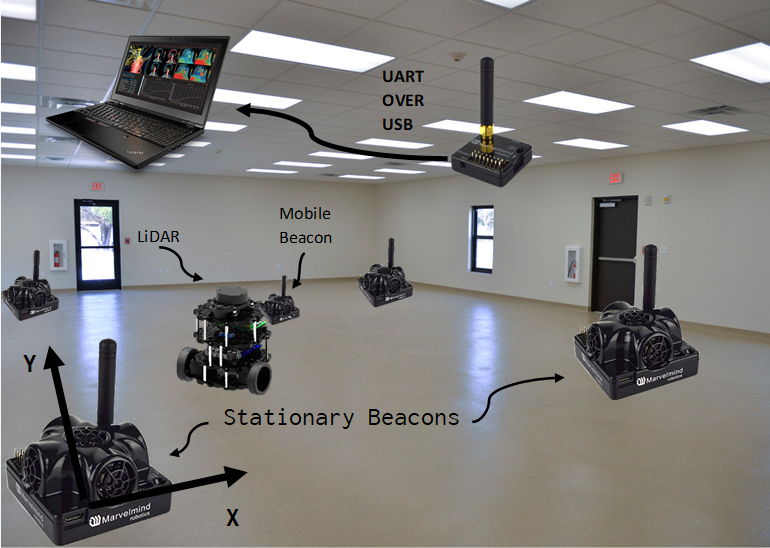
\includegraphics[width = \textwidth]{beacons.jpg}}
\end{figure}
\\The final test for Dr. McCourt will involve both the Marvelmind Beacons and 
LiDAR working in conjunction with the ORPS-Robot. We will define three criteria 
to get to this point. Those criteria will be defined bellow. This test will involve 
the ability to setup the Marvelmind sensors into a room in a rectangular fashion, with 
a mobile beacon on the ORPS-Robot. These sensors will be talking to each other. We will 
feed some desired path to the user to follow while the Marvelmind sensors measure the actual 
path that the robot is taking.
That error between what the user is doing and what the Marvelmind 
sensors are feeding back is what we care about. This is also where we will be testing the LiDAR. The 
LiDAR will be mapping out the room giving back additional location data for error correction. There 
are many systems talking to each other in this system, as can be seen in the figure above. A unit test 
must be written for McCourt's input-output transformations to ensure that the transforms 
were implemented correctly in the software and output the correct values. A lot of care must be paid in the 
calculations here and \href{http://numerical.recipes/}{\textit{Press's Numerical Recipes in C}} should be 
consulted early and often to ensure accuracy.\\\\\\
\begin{itemize}
    \item[RC1.] Research Entry Criteria - This is where we establish that the appropriate 
    documentation, design, and requirements information is available to begin testing 
    the final system and judge correct behavior. This doesn't have to be at the very end, 
    but it must be at a stage where we can test multiple systems interacting at once.
    \item[RC2.] Research Continuation Criteria - this defines those conditions and situations that must 
    prevail in the final research testing process to allow testing to continue smoothly and robustly, that 
    serves meeting our final goal. This is also where the main stage where keeping the bug backlog 
    and having unit tests that just work without much fiddling. At this stage we want to be fighting 
    with how to use the tool, not just getting the tool to work to begin with.
    \item[RC3.] Research Exit Criteria  - This is the criteria we must meet to determine when the project has completed 
    the main stage of testing of Dr. McCourt’s research interests. This means that no changes need to be made to 
    this completed part, except to address system test defects introduced by later stages of the project. 
    No crash, halt, panic, unexpected process termination, or other stoppages in completing this part. The research 
    portion must be self-encapsulated from other portions of the project as much as possible. We must be able to reach 
    demo day, having completed this portion of the project, and for it to just work on command.
\end{itemize}
\newpage
\subsubsection{System Test Items Table}
% Please add the following required packages to your document preamble:
% \usepackage{graphicx}
\begin{table}[htp]
\resizebox{\textwidth}{!}{%
\begin{tabular}{|c|c|c|c|c|c|c|}
\hline
\begin{tabular}[c]{@{}c@{}}System Test\\ Number\end{tabular} & \begin{tabular}[c]{@{}c@{}}Components\\ Involved\end{tabular} & \multicolumn{1}{l|}{\begin{tabular}[c]{@{}l@{}}Research\\ Criteria\end{tabular}} & \begin{tabular}[c]{@{}c@{}}Pass \\ Criteria\end{tabular}                                                                             & \begin{tabular}[c]{@{}c@{}}Fail \\ Criteria\end{tabular}                                                                                  & Overview                                                                                                                          & \multicolumn{1}{l|}{Criticality} \\ \hline
SYST1                                                        & H2,H8                                                         & \multicolumn{1}{l|}{}                                                            & \begin{tabular}[c]{@{}c@{}}rplidar returns\\ back no errors\end{tabular}                                                             & \begin{tabular}[c]{@{}c@{}}rplidar returns\\ back errors\end{tabular}                                                                     & \begin{tabular}[c]{@{}c@{}}rplidar is a\\ package for\\ testing the\\ LiDAR\end{tabular}                                          & \textcolor{green}{\textbf{S1}}                               \\ \hline
SYST2                                                        & H2,H8                                                         & \multicolumn{1}{l|}{}                                                            & \begin{tabular}[c]{@{}c@{}}The LiDAR\\ can sufficiently\\ scan a room and\\ map it\end{tabular}                                      & \begin{tabular}[c]{@{}c@{}}The LiDAR\\ cannot sufficiently\\ scan a room and\\ map it\end{tabular}                                        & \begin{tabular}[c]{@{}c@{}}Testing of the\\ LiDAR system \\ to see whether it\\ can map room\end{tabular}                         & \textcolor{yellow}{\textbf{S2}}                               \\ \hline
SYST3                                                        & H2,H8                                                         & \multicolumn{1}{l|}{}                                                            & \begin{tabular}[c]{@{}c@{}}The LiDAR can\\ return back the\\ speed\end{tabular}                                                      & \begin{tabular}[c]{@{}c@{}}The LiDAR\\ cannot return\\ back the speed\end{tabular}                                                        & \begin{tabular}[c]{@{}c@{}}Tests must be\\ run on the LiDAR\\ system to measure\\ if it can return \\ back the speed\end{tabular} & \textcolor{yellow}{\textbf{S2}}                               \\ \hline
SYST4                                                        & H2,H8                                                         & \multicolumn{1}{l|}{}                                                            & \begin{tabular}[c]{@{}c@{}}roscore ran without\\ any erros\end{tabular}                                                              & \begin{tabular}[c]{@{}c@{}}roscore returned \\ back errors\end{tabular}                                                                   & \begin{tabular}[c]{@{}c@{}}roscore is the init\\ function for ros\\ and acts as a sanity check\end{tabular}                       & \textcolor{green}{\textbf{S1}}                               \\ \hline
SYST5                                                        & H2,H8                                                         & \multicolumn{1}{l|}{}                                                            & \begin{tabular}[c]{@{}c@{}}The base-station \\ can sufficiently send \\ packets to the\\ ORPS-Robot \\ and are received\end{tabular} & \begin{tabular}[c]{@{}c@{}}The base-station \\ cannot\\ sufficiently send \\ packets to the\\ ORPS-Robot \\ and are received\end{tabular} & \begin{tabular}[c]{@{}c@{}}The base station\\ must be able to talk\\ to the ORPS-Robot\\ over the network\end{tabular}            & \textcolor{yellow}{\textbf{S2}}                               \\ \hline
SYST6                                                        & H2,H7                                                         &                                                                                  & \begin{tabular}[c]{@{}c@{}}The ORPS-Robot\\ can sufficiently send \\ packets to the\\ base-station \\ and are received\end{tabular}  & \begin{tabular}[c]{@{}c@{}}The ORPS-Robot\\ cannot\\ sufficiently send \\ packets to the\\ base-station\\ and are received.\end{tabular}  & \begin{tabular}[c]{@{}c@{}}The ORPS-Robot\\ must be able to talk\\ to the base station\\ over the network\end{tabular}            & \textcolor{yellow}{\textbf{S2}}                               \\ \hline
SYST7                                                        & H2,H8                                                         &                                                                                  & \begin{tabular}[c]{@{}c@{}}The ORPS-Robot\\ can execute\\ correct movement\\ instructions\end{tabular}                               & \begin{tabular}[c]{@{}c@{}}The ORPS-Robot\\ cannot execute\\ correct movement\\ instructions\end{tabular}                                 & \begin{tabular}[c]{@{}c@{}}Some testing must\\ be done to show that\\ the ORPS-Robot\\ can move as instructed\end{tabular}        & \textcolor{red}{\textbf{S3}}                               \\ \hline
SYST8                                                        & H7,H8                                                         &                                                                                  & The unit test passes                                                                                                                 & The unit test fails                                                                                                                       & \begin{tabular}[c]{@{}c@{}}Simple sanity unit\\ test of the \\ Marvelmind sensors\end{tabular}                                    & \textcolor{yellow}{\textbf{S2}}                               \\ \hline
SYST9                                                        & H8                                                            &                                                                                  & \begin{tabular}[c]{@{}c@{}}The GUI passes user\\ testing\end{tabular}                                                                & \begin{tabular}[c]{@{}c@{}}The GUI does\\ not pass user testing\end{tabular}                                                              & \begin{tabular}[c]{@{}c@{}}User testing must be\\ done on the GUI\end{tabular}                                                    & \textcolor{red}{\textbf{S3}}                               \\ \hline
SYST10                                                       & H8                                                            &                                                                                  & \begin{tabular}[c]{@{}c@{}}The GUI passes\\ injection testing\end{tabular}                                                           & \begin{tabular}[c]{@{}c@{}}The GUI does \\ not pass injection\\ testing\end{tabular}                                                      & \begin{tabular}[c]{@{}c@{}}An injection of \\ fake user inputs will be\\ sent into the GUI\end{tabular}                           & \textcolor{red}{\textbf{S3}}                               \\ \hline
SYST11                                                       & H8                                                            &                                                                                  & \begin{tabular}[c]{@{}c@{}}The GUI passes\\ tests of inputs\\ similar to user testing\end{tabular}                                   & \begin{tabular}[c]{@{}c@{}}The GUI fails\\ tests of inputs\\ similar to user testing\end{tabular}                                         & \begin{tabular}[c]{@{}c@{}}Bugs found in user \\ testing are simulated with\\ injection testing\end{tabular}                      & \textcolor{red}{\textbf{S3}}                               \\ \hline
SYST12                                                       & H2,H8                                                         & RC1                                                                              & \begin{tabular}[c]{@{}c@{}}The input-output\\ transforms return \\ the correct results\end{tabular}                                  & \begin{tabular}[c]{@{}c@{}}The input-output\\ transforms return \\ the incorrect results\end{tabular}                                     & \begin{tabular}[c]{@{}c@{}}The input-output\\ transforms of Dr.\\ McCourt's research\\ are tested\end{tabular}                    & \textcolor{red}{\textbf{S3}}                               \\ \hline
\end{tabular}%
}
\end{table}
\noindent This table will be split into different tables on further revisions. I reached the size limit for 
latex and I will split this up later. The hardware testing modes column need to be added to some of the future tables. 
Also a column for software levels.
- Jake.
\section{Approach}
\subsection{Special Tools}
Most special tools in this project will be software based. These tools will mostly be used for 
debugging, bug tracking, reproducibility, source control and catching memory leaks. These tools will include:\\
\begin{itemize}
    \item[1. ] GDB - For the portions of the project written in C the GNU Debugger will be used 
    in tracking down bugs. Generally speaking print statements will not be used. For instance, 
    catching problems with linkages of programs we write will be caught most likely by use of the debugger.
    \item[2. ] PDB - For the portions of the project written in Python the Python Debugger will be used 
    in tracking down bugs. Generally speaking print statements will not be used.
    For instance, inside of the GUI, which will mostly be written in Python, the PDB may be run 
    to find issues in the domain of possible inputs. 
    \item[3. ] Git - For bug tracking, reproducibility and source control Git will be employed.
    Two of our group members have been using Git regularly. We will need to make sure all the team 
    members are up to speed with the philosophy of minor branches, that merge into the main branch and 
    making sure that we all aren't too far from the main branch. 
    \item[4. ] Valgrind - A tool used for memory debugging, memory leak detection and profiling.
     For example Valgrind can tell us if at some point in our program we've done conditional 
     jumps based on uninitialized values with bad reads of memory. When used in conjunction 
     with GDB this gives us the tools to test our programs in ways that are not possible 
     without it.
\end{itemize}
\subsection{Training Required}
As mentioned in Special Tools we will need to make sure all users are up to speed with using Git
and making sure that all teammates buy-in to using debuggers regularly. This is where level 4 comes 
from the five levels of software testing. \\\\\\
To distinguish in training needed we will ask two sections and split into these key areas:\\
\begin{itemize}
    \item[Non-Expert:] Do you plan to only use the ORPS-Robot for path recognition testing?
    \item[Experts:] Do you plan on furthering research in the ORPS-Robot?
\end{itemize}
\subsubsection{Non-Experts}
Non-experts need to be given some prompt on how to control the robot via the controller or 
keyboard and how to read the commands from the GUI. Some of this training will be buried inside 
of the UI itself and using good design principles. Good design is in itself an act of communication.
Care will be paid into having a deep understanding of the type of user that uses our device.
Clever and sophisticated GUI solutions will be superseded by GUI solutions that are simple and solving 
\textit{the correct problem}. 
\subsubsection{Experts}
Experts will need some prior knowledge in how to run each subsystem, as follows:\\
\begin{itemize}
    \item[1.] Having some knowledge of ROS commands. We will include a setup ritual for setting the project 
    up to where we leave it at.
    \item[2.] Having some knowledge of the Linux Ubuntu command line for running programs. We will 
    include some examples of this process to help the future users along.
    \item[3.] Having knowledge of setting up the Raspberry Pi and OpenCR to connect each component together, 
    also connecting the LiDAR to the robot. This will involve some sort of setup ritual that we will include.
    \item[4. ] Having the ability to follow a setup ritual we create for the Marvelmind sensors.  
\end{itemize}
For experts some self-learning will be required as we cannot possibly include all cases that need to be covered 
but some baseline of the setup ritual process will be passed onto the next group for further research purposes.
\subsection{Metrics}
\subsubsection{Metrics Methodology}
Our tests will be derived from the requirements and specifications of our project and will follow 
the following methodological approach:
\begin{itemize}
    \item[T1.] Acceptance Testing: Assess system (software \& hardware) interaction with respect 
    to user needs. For example, making sure the controller is responsive or camera is functioning 
    adequately.
    \item[T2.] System Testing: Assesses system interaction to architecture design and overall behavior. 
    For example a series of rostests that test the linking of each submodule we write for the overall 
    project.
    \item[T3.] Integration Testing: The continuous conjoining of different software artifacts to 
    serve the overall project development. For example, a test that ensures two individual modules are 
    linked properly.
    \item[T4.] Unit Testing: Assesses system interaction with respect to implementation of specific subsystems. 
    For example, a test that ensures the controller is functioning properly standalone through the joy 
    package.
\end{itemize}
While these levels are emphasized in terms of when they are applied, it is more important to distinguish 
the types of faults listed above. They are all a continuous part of the design and build process. At 
the end of the day there is an entire spectrum of testing, and much of it is hard to distinguish from 
development itself. Most tests look like unit tests and are quite simple. Other tests are more subtle, 
complex and critical. For such tests we need to use the tools laid out in this document to check our 
implementation. In the testing process the standard behavioral model should be employed, where 
execution of a program or task is represented by a behavior. A behavior is sequence of states while a state 
is an assignment of values of variables. Our program should be tested and modeled by a set of behaviors 
we define, representing possible executions. 
\subsubsection{Measuring Safety}
Safety when testing can be specified using two things:\\
\begin{itemize}
    \item[-] The set of possible initial states.
    \item[-] A next-state relation, describing all possible successor states of any state. 
\end{itemize}
The above is a mindset that integrates the testing process into the development process.\\\\\\
Failures can rarely be forecasted. But what we can do is establish a hierarchy of 
criticality to ensure that we are keeping up with the most important test and using 
other tests as needed. Ordering what we need to do by priority is important as the scope 
of the project grows. The reason for the priority emphasis is that it is by far 
the most efficient way of working, in terms of creating reliable products and reducing 
the overall cost of the project. For instance using the wrong battery on the ORPS-Robot 
would likely ruin at least the Raspberry Pi or OpenCR, along with other mission critical 
components. This is not only a likely outcome if special care is not paid but we have seen it 
happen with prior groups in previous projects in this program. For this reason a heavy emphasis 
will be paid on this scheme.
\subsubsection{Criticality}
\begin{figure}[h!]
    \centerline{
\includegraphics[width = \textwidth]{crit.jpg}}
    \caption{The \textit{Criticality} hierarchy for the ORPS-Robot}
\end{figure}
\begin{itemize}
    \item[S1.] Secondary Service - These involve services that are only checked when a component 
    fails. Use see in many applications test conditions can take longer to create than others. 
    This is the sort of service that happens ala cart and may be indistinguishable from the actual 
    build and design process in spots. These are components that we should likely assume work until 
    they don't.
    \item[S2.] Critical or Primary Service - Most component tests, both software and hardware, 
    fall under this category. Some but not all integration test that fall under interaction of 
    components (system test items) will likely fall under this category. These are services that 
    if they fail, will not mean the end of the project, but are extremely critical components 
    and should be worried about early and often.
    \item[S3.] Mission Critical Service - Most acceptance tests will fall under this category, this 
    means systems test items critical to Dr. McCourt’s research and of our object recognition 
    portion. A lot of integration testing will follow under this category. These are services 
    that if they fail, then the project has serious issues that need to be resolved.
\end{itemize}
\subsubsection{Regression Testing}
In this section we will discuss three criteria for regression testing on the ORPS-Robot platform. 
That is answering three key questions:\\
\begin{itemize}
    \item[1.] What kind of tests should be in a regression test for this project?
    \item[2.] When to run regression tests?
    \item[3.] What to do when a regression test fails? 
\end{itemize}
Research criteria testing should part of the regression testing, as those are tests, that must not introduce 
bugs once implemented as those are the most critical tests for the project. GUI testing and unit tests 
must be part of the regression testing. The logic for including these in regression testing is as follows: 
these are the tests of the most critical sections of the project as such follows the criticality hierarchy. 
It can be assumed that most secondary and critical or primary services can be assumed to be working once tested 
and shown to be working. The mission critical services for this project tend to be the most forward facing, as they 
serve the point of interaction between the user either in form of the research interests or the graphical user interface. 
Including every test imaginable in the regression testing is undesirable and only these tests will be done on regular intervals.\\\\
As for when the regression tests will be done whenever a new functionality is introduced to the 
project. Since we will be doing issue tracking for defect detection this will make sense to do so, and should create a tight enough 
loop of creation, integration then testing. If a regression test fails it will be up to the developer implementing the change to either 
get in contact with the developer who's section of the project is broken to know to fix it or to fix it themselves. This will be up to the 
developer who discovers the fix to decide. Regression testing should be \textbf{modification-revealing}, \textbf{precise}, 
\textbf{efficient} and \textbf{general}. Techniques like data flow were not used in selecting tests for regression testing 
because it is neither \textbf{safe} or \textbf{precise}. Critical thinking was used in the selection process. 
\section{Fail Criteria \& Testing Deliverables}
The main deliverable for this project is a platform to aid in research. By the end of this project there 
must exist an artifact to aid and abet network control systems research. To accomplish this goal we must 
build a platform that allows a user to control a robot and collect the data of the user using the robot. 
Testing is an area where a lot can go wrong and Murphy's Law is in full effect: if something can go wrong, 
it will. We will accomplish testing our deliverables by following this checklist:\\
\begin{itemize}
    \item[1.] Is the deliverable working as originally designed?
    \item[2.] Are the identified operational requirements being met?
\end{itemize}
The decision of whether we've failed to meet the research criteria as defined in the above regression testing section 
will be a pass or fail decision decided by our client. This fail criteria, while crude, avoids the IEEE 826 format 
that requires failure criteria being centered around defects as it is becoming exceedingly clear that identifying and cataloging 
defects is exceedingly intractable. This criteria was clearly defined for projects for large teams with the resources to do so. Instead 
a more tractable and punitive failure criteria will be adopted. If it becomes clear the defects are a part of this project in the future 
and that we can catalog them effectively then a defect detection percentage will be used to measure success in dealing with them.
\subsection{Defect Detection Percentage}
This metric will be using is the \textit{defect detection percentage} on testing the research portion of this project. 
We will define this metric as follows:\\\\
\centerline{$\text{DDE} = \frac{\text{Bugs Prior to Research Testing}}{\text{Bugs Prior to Research Testing} + \text{Bugs during Research Testing}}$}
\\\\
Bugs are required to be unique for the relationship in this equation to hold, but if they are the DDE should 
give us some sort of metric on how well we captured and tackled bugs prior to release. This 
assumes for the sake of argument that all bugs are \textit{ceteris paribus} (all things held equal).
This is not the case. All bugs are not created equal, neither are all metrics, but they do 
allow us some sort of evaluation on our quality of work.\\\\
\section{Roles}
Roles will be split up according to their need. Since this is not much of a hardware project, 
the role of hardware test items will fall under the purview of Alex. For the software and 
system test items, those will be split among all three members. All three members will need to 
be familiar with the tools listed in the special tools section. All three group members in the 
ORPS-Robot group will be writing code, which means debugging code. Jake will focus on the 
Marvelmind sensors testing for trilateration, Ammon will focus on testing the path smoothing, 
and Alex will focus on testing the GUI. These roles are subject to change with time but this is 
the current understanding of who's roles are what. There should be overlap with each role and 
it should be no one person's role to do all of one thing if the work grows in complexity. Alex's 
job will be keeping track of the schedule, Jake's job will be keeping track of bugs in some sort of 
process, and Ammon's job will be to manage the git repository to make sure all branches are integrating 
smoothly.
\section{Schedule}
\subsection{Delay Handling}
In the testing of the different components of the final system there are always possibilities 
for unpredictable delays in the schedule, caused by either the testing or by the design. 
To stop these delays from having an effect on the overall project completion time there are a 
couple safeguards in place to ensure the project remains on schedule.\\\\
The first safeguard in place is the breaks in between quarters. In the estimation for 
completing specific tasks, the breaks between quarters was not included as optional time. 
This allows for two, 2 – 3 weeks of time, which are completely clear of other curricular 
activities, to catch up on the schedule or to get ahead.\\\\
If the breaks in between quarters are not enough time to handle the delays the first task 
besides stretch goals which will be allowed to be shortened or removed, is the testing of 
the radar sensor. The completion of the Marvelmind positional sensors is necessary for the 
testing of input-output transform, so the robot’s primary purpose will still be able to 
function without a completely tested radar system. The image recognition is not necessary for this project 
and therefore will be cut if time does not allow it.
\subsection{Dates}
\begin{itemize}
    \item[] Testing controller functionality: Dec-$8^{th}$ to Jan-$7^{th}$
    \item[] Testing moving robot with controller: Jan-$7^{th}$ to Jan-$21^{st}$
    \item[] Testing Marvel Mind position sensors: Feb-$7^{th}$ to Feb-$14^{th}$
    \item[] Testing moving the robot to positions using the sensors: Feb-$21^{st}$ to Feb-$28^{th}$
    \item[] Testing Testing the input-output tranformation: March-$21^{st}$ to March-$28^{th}$
    \item[] Testing algorithm implemented in the system: April-$7^{th}$ to April-$14^{th}$
    \item[] Testing Lidar room mapping functionality: April-$21^{st}$ to April-$28^{th}$
    \item[] Testing Intel RealSense camera: May-$1^{st}$ to May-$7^{th}$
    \item[] Testing Image and object recognition: May-$14^{th}$ to May-$21^{st}$ 
\end{itemize}
\section{Testing Risks and Mitigation}

\section{Approvals}

\end{document}